%!TEX root = ../paper.tex

\section{Introduction}
\label{sec:introduction}

Recent years have shown a trend for companies from buying standalone software with big service contracts to buying small cloud products, also known as software as a service (SaaS).
Software is licensed on a subscription and per-use basis and is hosted on the vendors's servers.
Vendors of such software are now able to set the subscription fees dynamically according to usage time, company size, or revenue.
For the customer companies, this approach allows to scale easily when the company grows or declines or does not need the services for a certain time span.

These new possibilities increased the set of potential customers for software vendors.
As Dubey and Wagle~\cite{dubey2007delivering} said, ``buyers have more flexibility to switch vendors and perhaps fewer headaches in maintaining the software''.
Especially young companies are more likely to buy SaaS, as it gives them the flexibility to adapt to the growth of the company in the future.
So, rather than being restricted to a small range of companies, for example only big enterprise companies or only young startups, vendors can sell their products to all kinds of companies.
However, this change introduces a new problem for salesmen: due to the sheer amount of possible customers, salesmen cannot contact all companies in the market, because this would be an infeasible task.
Rather, they want to find those companies, who are likely to buy one of their products.
When only a few companies are available, salesmen can just inquire personally and try to sell their products.
In the new setting, it becomes harder and more time-consuming to find potential customers.

We propose a new approach to find potential customers by automatically recommending users, who ask for product recommendations in social networks.
Social networks are platforms, where users can post status updates, ask questions, start discussions, or receive recommendations.
A special type of social network, so called business-oriented social networking services, such as LinkedIn\footnote{http://www.linkedin.com/} or Xing\footnote{http://www.xing.com}, especially lend themselves to building business relations and asking for professional advice.
There, users ask for opinions and recommendations on products.

This offers a huge possibility for companies to identify potential buyers.
Rather than booking advertising time in television or advertising banners on news websites, they can target their salesman on persons, who are more likely to buy a product.
As Mobasher et~al.~\cite{mobasher2007toward} state, ``it is a basic truism from marketing, that it is best to target those potential customers, who are already predisposed towards the product''.

Thus, it makes sense for companies to find these people looking for advice.
However, the large amount of daily status updates makes it infeasible to identify these posts manually.
According to LinkedIn, there were 186 million unique monthly visitors in 2013\footnote{http://blog.linkedin.com/2014/05/01/linkedins-q1-2014-earnings/}. 
39~\% of them post status updates regularly.
% http://www.forbes.com/sites/cherylsnappconner/2014/05/04/new-research-2014-linkedin-user-trends-and-10-top-surprises/
This sheer amount shows, that technical assistance is needed.

At the moment, the process of finding relevant status updates mostly happens by providing a search engine on the posts.
Salesmen need to manually find good search terms, enter them in the network's search field and then scan the results for potential buyers.
This approach requires expertise on the hand of the salesmen to find good search terms and tweak them accordingly.
Furthermore, scanning through the result lists is cumbersome and tedious.
Also, it is simply impossible to search through a large set of posts, say over a million, and find the best possible customers, where best means that there is a high probability of a deal.

We propose an approach, which is based on automatic text classification to identify relevant posts for a salesman.
Therefore, we employ techniques of supervised machine learning to categorize posts.
We call our approach \emph{noise to opportunity}, as we automatically filter the best selling opportunities from the large and diverse set of potential social network posts.

To classify posts, the machine learning requires to have labeled posts to use as training data for the learning algorithm.
As this training data does not exist, it would need to be created manually by the salesmen.
However, this is not feasible for a company, as it takes precious time for tagging post from the salesmen, in which they could actually sell products.
Therefore, we propose an approach, which automatically uses the company's brochures and advertising texts for learning.
A company usually has some set of advertising material, flyers, or presentation slides, where they promote their own products.
Based on this material, we automatically learn to distinguish between products, and then propose posts with selling opportunities to the salesman.
The architecture of our system is illustrated in Figure~\ref{fig:figureone}.


\begin{figure}
	\begin{center}
		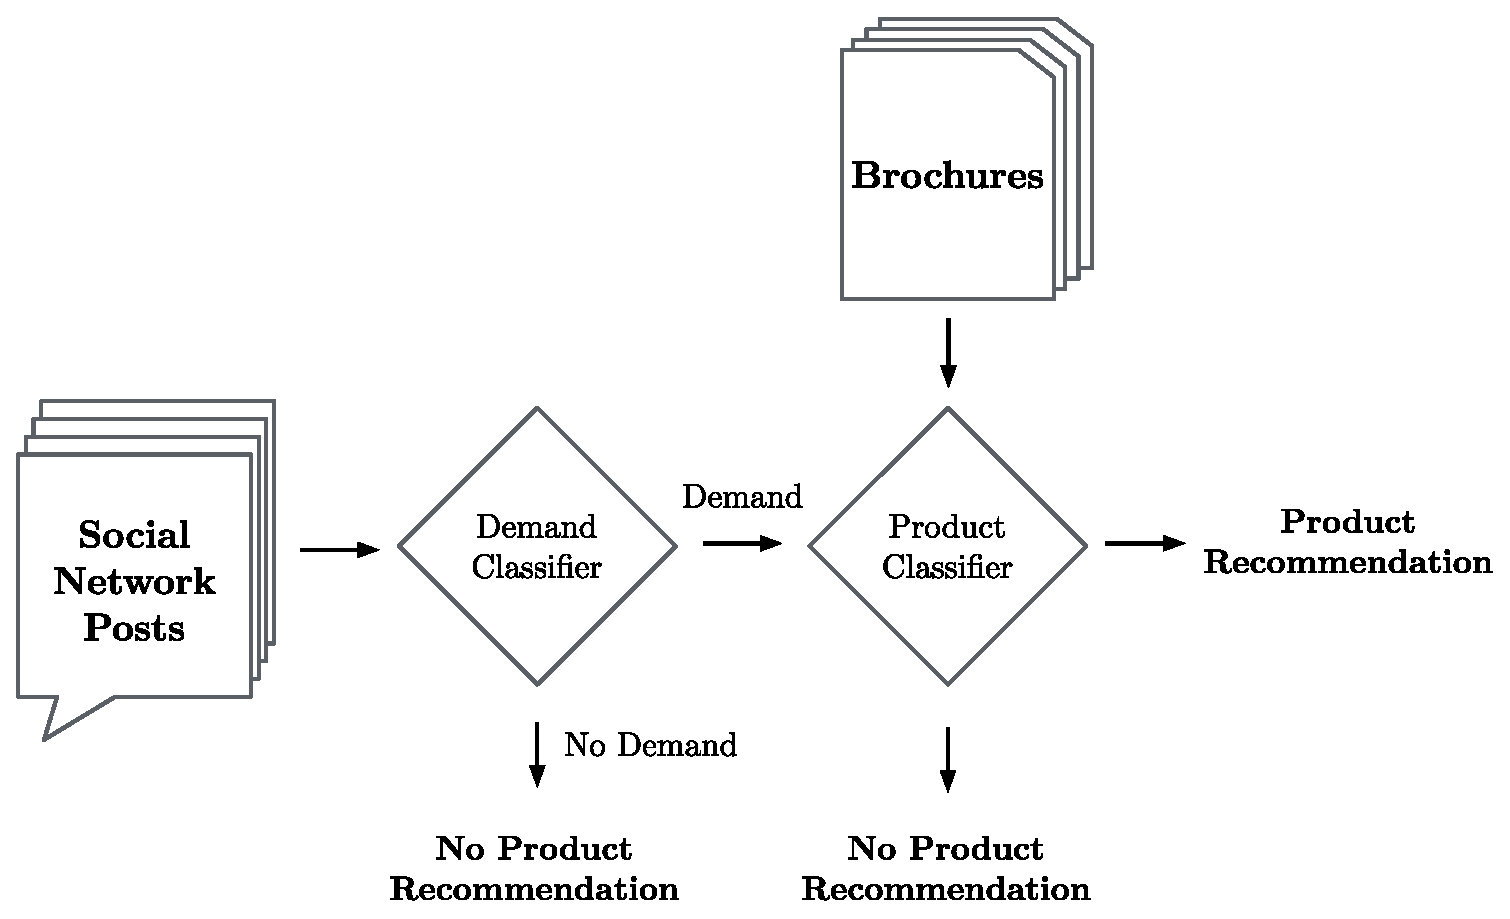
\includegraphics[width=0.7\textwidth]{figures/nto_workflow.eps}
	\end{center}
	\caption{Together, a demand classifier trained from social network posts and a product classifier trained from marketing material form a classification-model for unseen posts.}
	\label{fig:figureone}
\end{figure}

Yet, this approach introduces new problems.
Firstly, there are not many documents to learn from.
The number of brochures per product is usually far below one hundred.
To overcome this small corpus problem, we employ feature selection to select only the most relevant words and ignore the noise.
Secondly, if a user posts something about a certain product, this does not automatically allow the conclusion, that the user is actually interested in buying the product.
Therefore, we introduce a two-stage classifier, which first determines the demand of a user, and then determines, whether the user posts about a product.
This approach allows to capture, whether the user actually needs the product.

Section~\ref{sec:background} gives a formal problem definition and shows related work.
Section~\ref{sec:concept} shows our two-stage classification approach and how we use feature selection to overcome the small corpus problem.
Section~\ref{sec:implementation} shows the implementation of both the demand and the product classifier.
It also presents the best configuration for the algorithm.
In Section~\ref{sec:evaluation}, we evaluate our approach.
Section~\ref{sec:conclusion} summarizes and shows future work directions.
